\section{Relative Error and Graphic Analysis}
\label{error}

\subsection{Frequency Response Analysis}
\label{subsec:freqresp}

\paragraph{}
A frequency response analysis was performed using both NGSpice for simulation interpretation and GNU Octave for theorethical analysis. The graphics ploted by each one of the tools are, as we can see, very similar to eachother. Once again, it is a confirmation of the good results that we were able to obtain during the implementation of both the circuit simulation and the theoretical analysis perfomed with GNU Octave.

\begin{figure}[H]
\begin{subfigure}{0.5\textwidth}
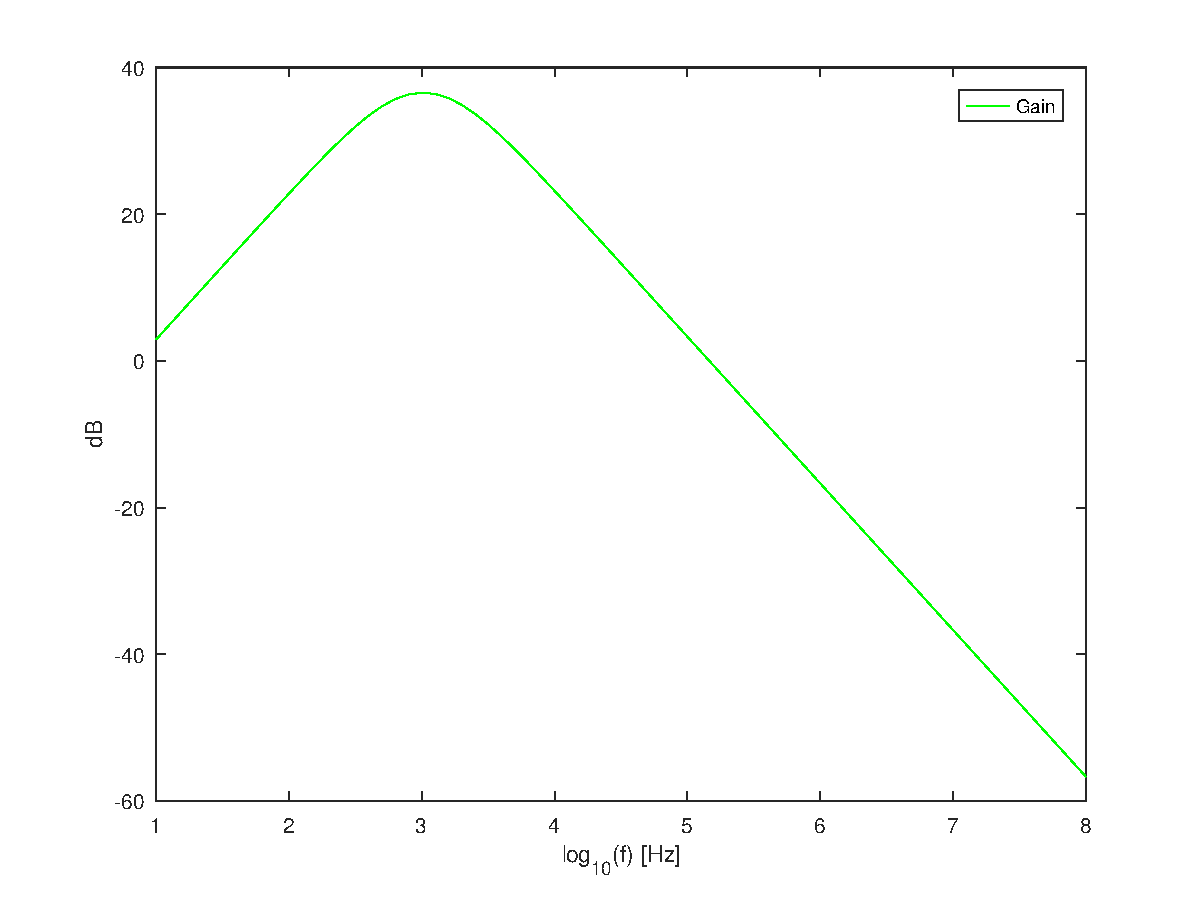
\includegraphics[width=0.9\linewidth, height=8cm]{theo.eps} 
\caption{The Theoretical frequency response - gain[dB], obtained using GNU Octave.}
\label{fig:theo_third}
\end{subfigure}
\begin{subfigure}{0.5\textwidth}
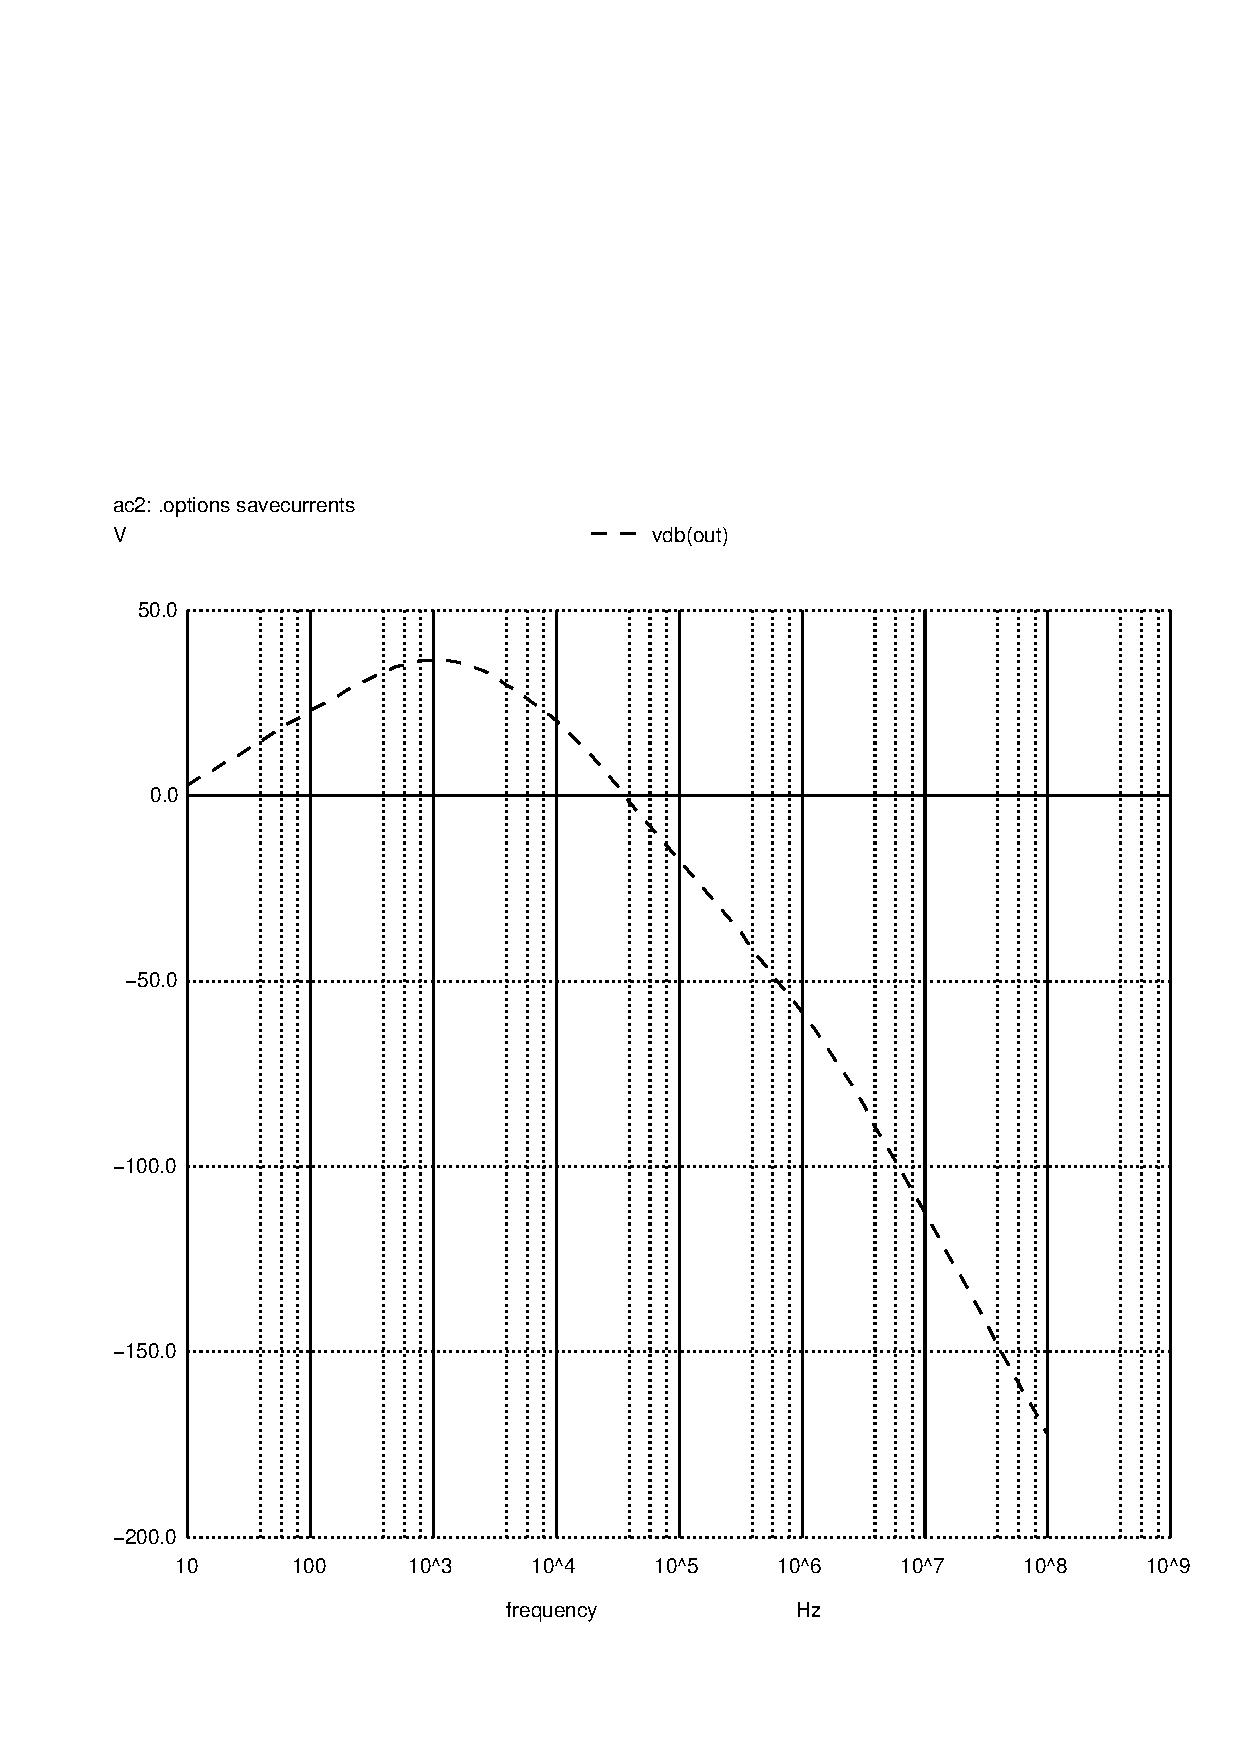
\includegraphics[width=0.8\linewidth, height=8cm]{gain.pdf}
\caption{The Simulated frequency response - gain[dB], obtained using NGSpice.}
\label{fig:total}
\end{subfigure}
\end{figure}

Taking a closer look at both figures side by side, we can see that they are, in fact, very similar. The only small difference we can find is, by taking a closer look, that they have different values for the maximum voltage gain, even though both are very close to the required 40 dB. A quick explanation for this small error is that, while in Octave we use an ideal OP-AMP model, NGSpice uses a real OP-AMP model, that takes into account that the output impedance is not null.

\begin{figure}[H]
\begin{subfigure}{0.5\textwidth}
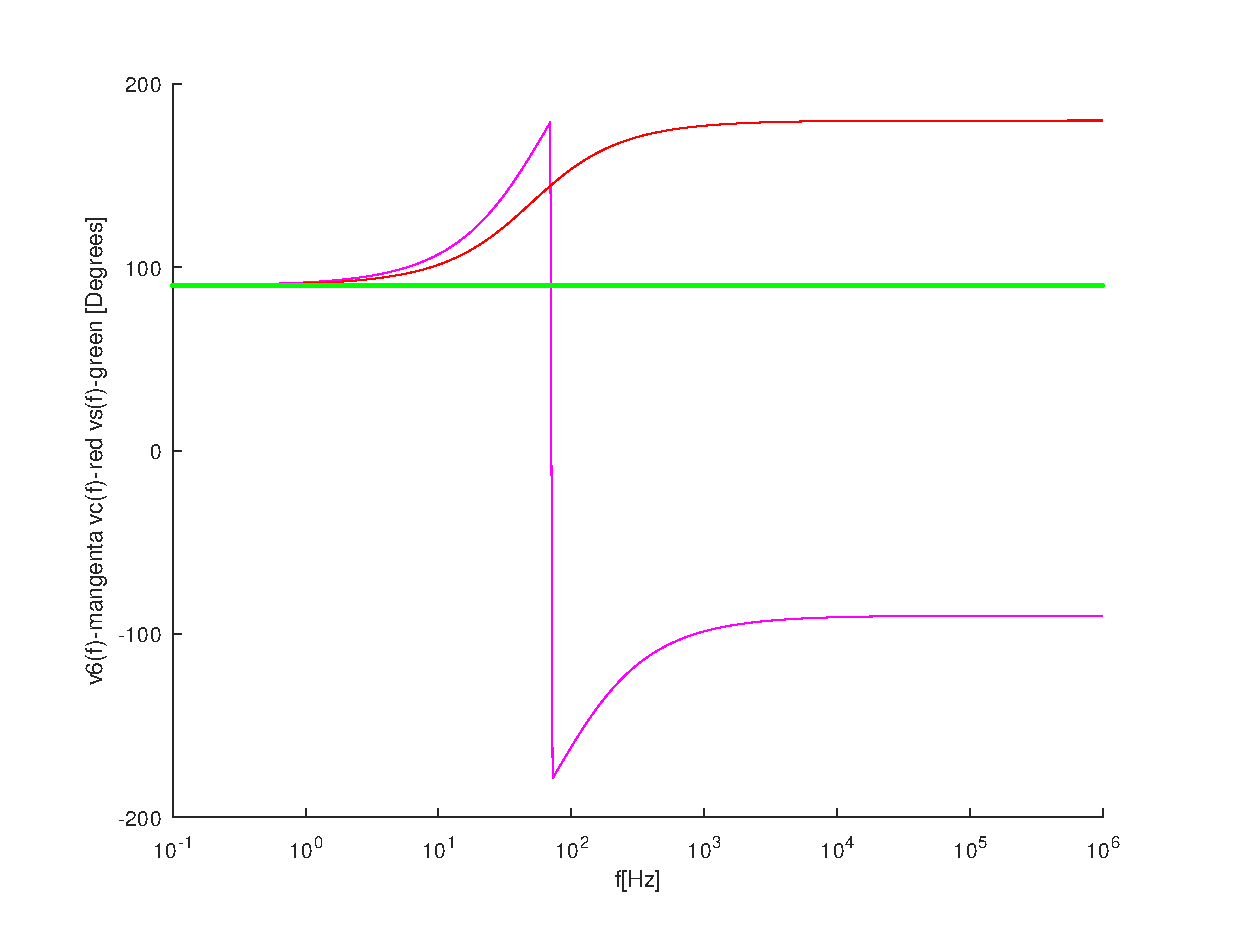
\includegraphics[width=0.9\linewidth, height=8cm]{phase.eps} 
\caption{The Theoretical frequency response - phase[deg], obtained using GNU Octave.}
\label{fig:theo_fourth}
\end{subfigure}
\begin{subfigure}{0.5\textwidth}
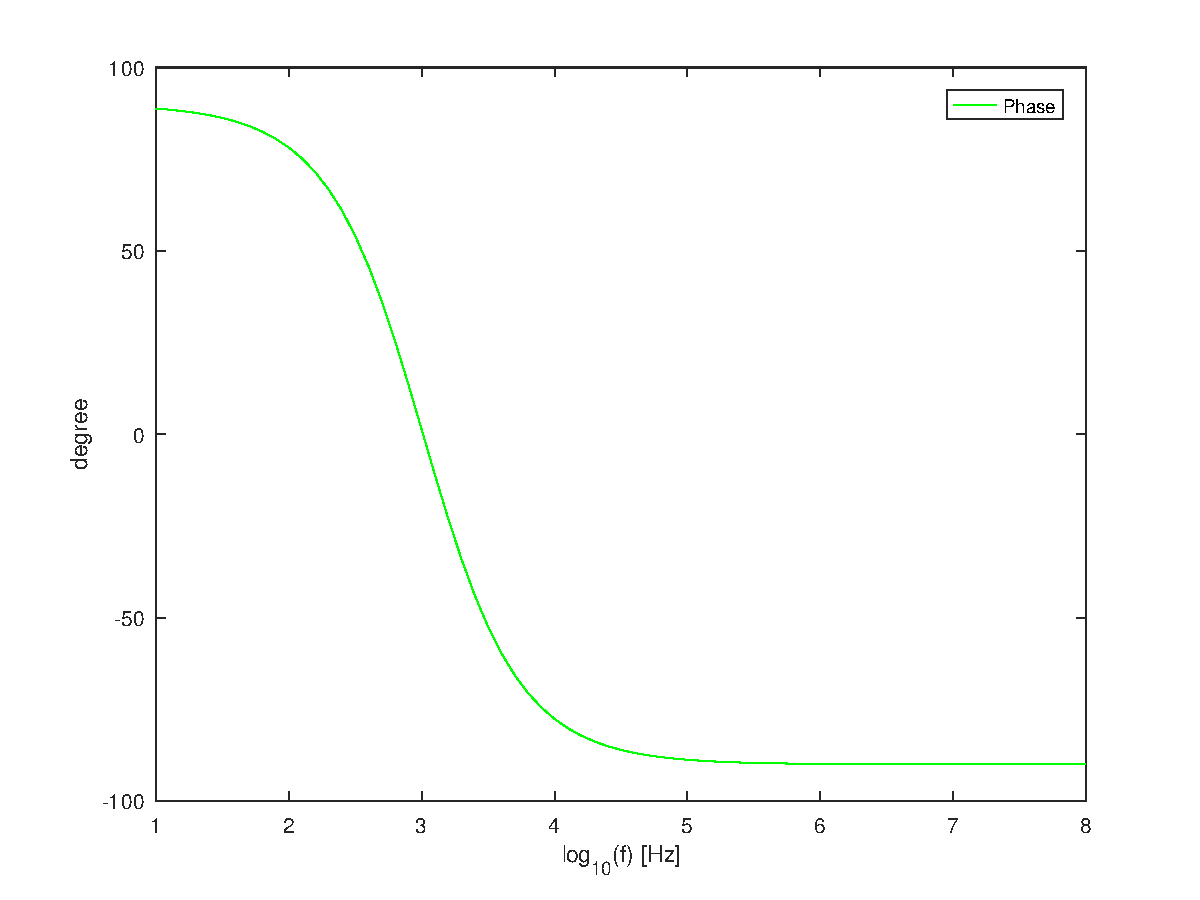
\includegraphics[width=0.8\linewidth, height=8cm]{phase.pdf}
\caption{The Simulated frequency response - phase[deg], obtained using NGSpice.}
\label{fig:theo_fifth}
\end{subfigure}
\end{figure}

Once again, we can see that both figures are very similar to eachother.

\begin{center}
   \begin{table}[H]
\resizebox{\textwidth}{!}{%
\begin{tabular}{|c|c|c|c|c|}
\hline
& \textbf{NGSpice Value} & \textbf{Octave Value} & \textbf{Relative Error} & \textbf{Percentual Error {[}\%{]}} \\ \hline
Gain & 67.0836 V & 67.3177 V & $3.489675569 \times 10^{-3}$ & 0.3489675569 \\ \hline
Gain dB & 36.5323 dB & 36.5626 dB & $3.294030214 \times 10^{-4}$ & 0.08294030214 \\ \hline
Lower Cut-Off Frequency & 406.808 Hz & 398.107 Hz & 0.02138846827 & 2.138846827 \\ \hline
Higher Cut-Off Frequency & 2481.27 Hz & 2511.886 Hz & 0.01233884261 & 1.233884261 \\ \hline
Central Frequency & 1004.69 Hz & 1000 Hz & $4.66810658 \times 10^{-3}$ & 0.466810658 \\ \hline
Bandwidth & 2074.46 Hz & 2113.779 Hz & 0.01895384823 & 1.895384823 \\ \hline
Input Impedance & 1234.29 Ohm & 1234.242 Ohm & $3.888875386 \times 10^{-5}$ & $3.888875386 \times 10^{-3}$ \\ \hline
Output Impedance & 824.902 Ohm & 822.637 Ohm & $2.745780711 \times 10^{-3}$ & 0.2745780711 \\ \hline
\end{tabular}%
}
\end{table}
\end{center}

\paragraph{}
In the table above, we have the comparison between the values obtained using Octave and NGSpice. Both the relative error and percentual error are included to make the interpretation easier. 

\paragraph{}
Even though most of the erros presented are really small, which proves the accuracy of the results obtained, these small discrepancies can be explained by the fact that, when we use GNU Octave, we are considering an ideal OP-AMP model, which assumes that the output impedance is zero. In fact, it´s not zero, and NGSpice uses a model that takes that into consideration, and so these differences between the models used by both NGSpice and Octave are, most likely, the main factor of the errors observed. 

\subsection{Figure of Merit}
\label{subsec:Figure_of_Merit}


\paragraph{}
To end our report, we present the figure of merit. It is important to remind that this figure is obtained upon the devices and values used in Ngspice. During our work, we have performed several incremental modifications to improve the merit figure.

\begin{center}
   \begin{tabular}{|c||c|}
      \hline    
      \multicolumn{2}{|c|} {\bf Figure of Merit and Cost} \\
      \hline
      Cost & 13426.7 MU \\ \hline
      Merit & $9.12982 \times 10^{-6}$ \\ \hline
   \end{tabular}
 \end{center}
 
\paragraph{}
The variation of these parameters allowed us to achieve an improved figure of merit, while trying to obtain the required parameters (the central frequency and the gain at the central frequency) and to minimize the cost of the circuit's components. The values applied both in NGSpice and Octave proved to be our best options to make the figure of merit as high as possible, even though the results obtained seem a bit lackluster.
